\section{Experimental Setup}\label{app:exp_setup}

\begin{figure}[htbp]
    \centering
    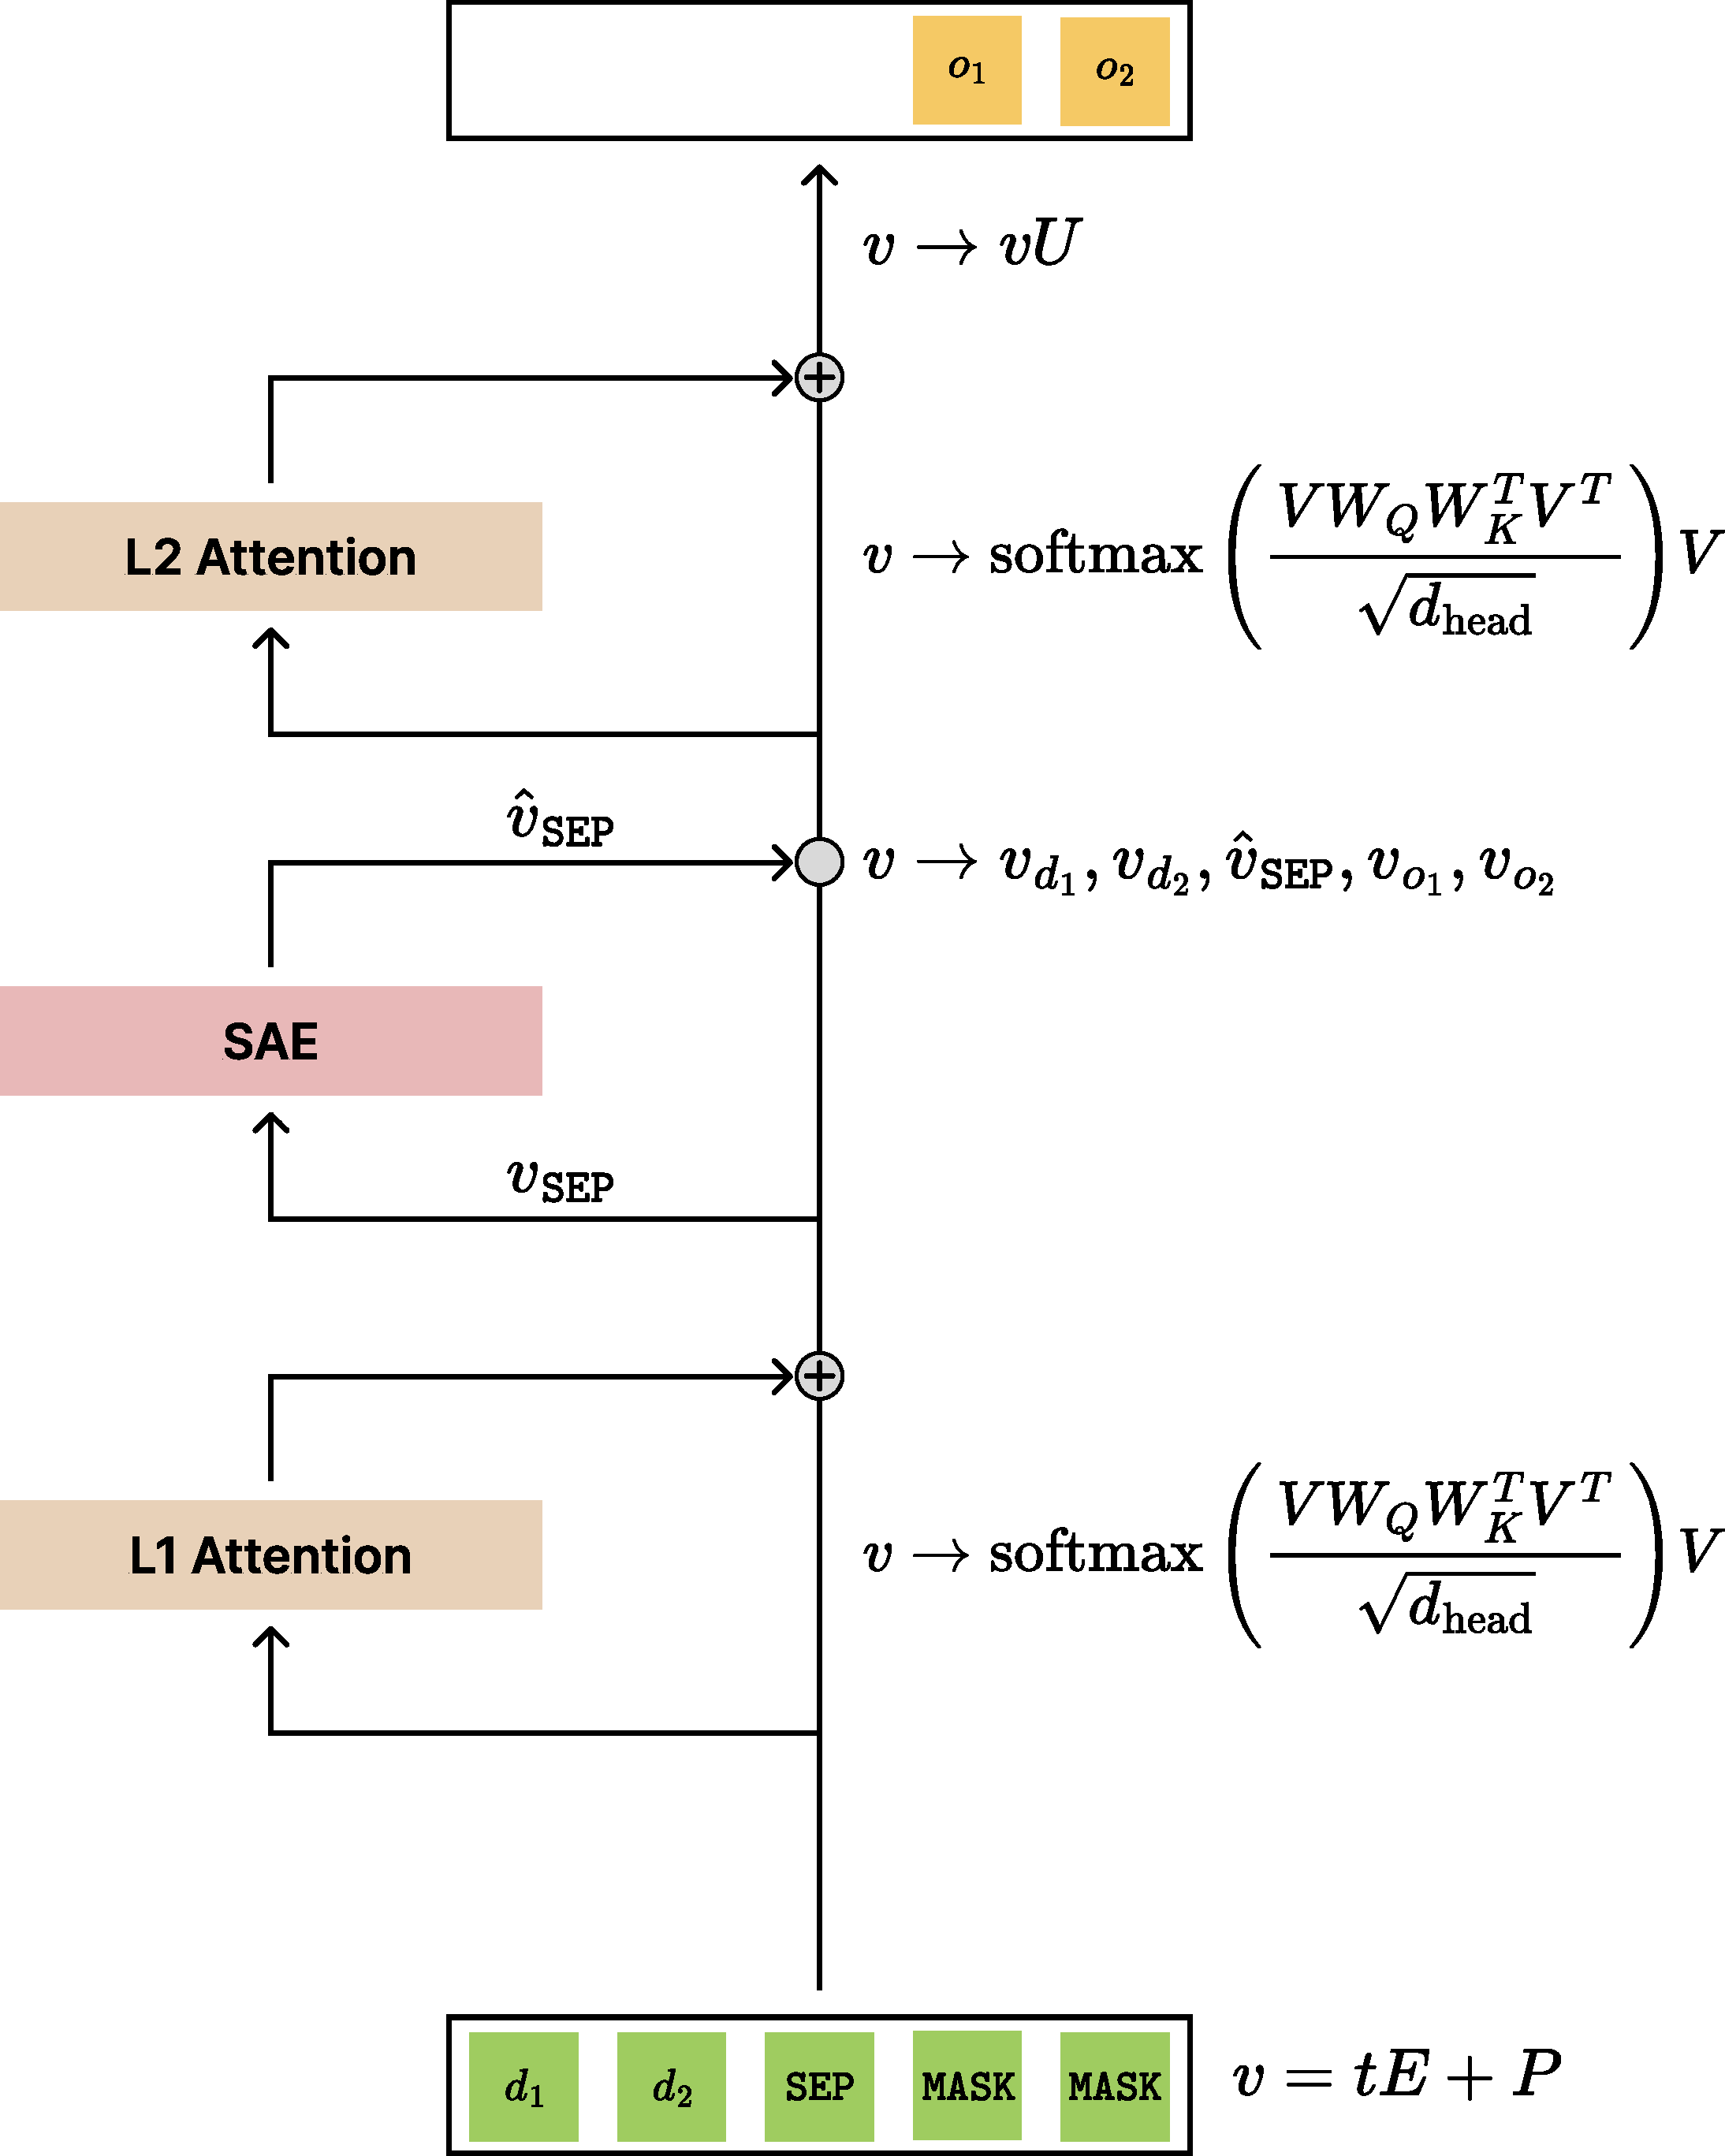
\includegraphics[width=0.5\linewidth]{figures/rq2_pipeline.pdf}
    \caption{
      This diagram shows the structure of the two-layer attention-only transformer and how the SAE is used to extract and analyse the learned representations. $v$ denotes the residual stream, which is read from and written to after each layer and has shape $(5,d_\text{model})$. $t$ is the vector of input tokens $[d_1, d_2, \texttt{SEP}, \texttt{MASK}, \texttt{MASK}]$, $E$ and $P$ are the token and position embedding matrices respectively, $U$ is the unembedding matrix, and each attention layer has key and query matrices, $\boldsymbol K^i$ and $\boldsymbol Q^i$ respectively, for $i \in [1,2,3]$. The value and output matrices for each layer are fixed to the identity, and $d_\text{head}=64$.
      The SAE takes the residual vector at \texttt{SEP}, $v_\texttt{SEP}$, as input and patches reconstruction $\hat{v}_\texttt{SEP}$ back into the stream.
      Accuracy is calculated on the final two output logits only, represented by $(o_1, o_2)$.
    }
    \label{fig:rq2_pipeline}
\end{figure}

\begin{table}[htbp]
\centering
\caption{
SAE hyperparameter sweep configurations. Braces denote swept values; fixed values are listed directly.
Fixed parameters across all runs: 50{,}000 training steps, 1{,}000 warmup steps, 4{,}096 batch size.
Total run counts are the product of all swept values and seeds. Note that $n_\text{groups}=1$ in a Matryoshka SAE reduces it to a standard BatchTopK SAE, so this serves as an internal consistency check.
}
\label{tab:sae_sweep_configs}
\resizebox{\linewidth}{!}{%
\begin{tabular}{ll}
\toprule
\textbf{Parameters} & \textbf{Swept Values} \\
\midrule
$d_{\mathrm{SAE}}$ & \{128, 192, 256, 320\} \\
$k$ / Target $L_0$ (All) & \{3, 4, 5\} \\
$k$ / Target $L_0$ (BatchTopK extra) & \{1, 2\} \\
$k$ / Target $L_0$ (JumpReLU extra) & \{2\} \\
JumpReLU sparsity penalty & \{0.1, 0.5, 1.0, 5.0\} \\
JumpReLU learning rate & \{$7\!\times\!10^{-5}$, $3\!\times\!10^{-4}$\} \\
BatchTopK, Matryoshka learning rate & $3\!\times\!10^{-4}$ \\
Matryoshka $n_{\text{groups}}$ & \{1, 2, 4\} \\
\midrule
& \textbf{Seeds / Total Runs} \\
\midrule
BatchTopK & 15 seeds / 450 runs \\
JumpReLU & 5 seeds / 640 runs \\
Matryoshka & 15 seeds / 540 runs \\
\bottomrule
\end{tabular}
}
\end{table}
% NOTE maybe each SAE should have equal number of runs to avoid bias in aggregate stats?

\begin{table}[ht]
\centering
\caption{SAE sweep results aggregated over multiple seeds (mean $\pm$ std). $L_0$: mean active features per token. $d_\text{SAE}$: dictionary size. \textbf{LR} (loss recovered): fraction of model loss recovered by the SAE reconstruction ($\uparrow$ better). \textbf{Dead\,\%}: percentage of dictionary features with zero activation across the evaluation set ($\downarrow$ better).
\textbf{Bold}: best within each $L_0$ block; \underline{\textbf{underlined}}: best overall.}
\label{tab:sae_sweep}
\begin{tabular}{ccrr}
\toprule
$L_0$ & $d_\text{SAE}$ & Runs & LR ($\uparrow$) & Dead \% ($\downarrow$) \\
\midrule
  1 & 128 & 44 & $0.9368 \pm 0.0028$ & \textbf{13.5 $\pm$ 2.1} \\
  1 & 192 & 15 & $\mathbf{0.9410 \pm 0.0014}$ & 43.9 $\pm$ 1.9 \\
  1 & 256 & 15 & $0.9406 \pm 0.0011$ & 53.9 $\pm$ 2.0 \\
  1 & 320 & 15 & $0.9397 \pm 0.0015$ & 61.9 $\pm$ 1.3 \\
\midrule
  2 & 128 & 57 & $0.9798 \pm 0.0101$ & \textbf{17.0 $\pm$ 2.6} \\
  2 & 192 & 20 & $0.9835 \pm 0.0056$ & 43.7 $\pm$ 2.2 \\
  2 & 256 & 20 & $\mathbf{0.9836 \pm 0.0048}$ & 55.8 $\pm$ 2.7 \\
  2 & 320 & 20 & $0.9828 \pm 0.0051$ & 63.2 $\pm$ 3.1 \\
\midrule
  3 & 128 & 405 & $\mathbf{0.9984 \pm 0.0036}$ & \textbf{17.4 $\pm$ 2.8} \\
  3 & 192 & 293 & $0.9984 \pm 0.0020$ & 41.1 $\pm$ 3.8 \\
  3 & 256 & 195 & $0.9979 \pm 0.0023$ & 51.5 $\pm$ 6.0 \\
  3 & 320 & 201 & $0.9979 \pm 0.0024$ & 57.7 $\pm$ 7.4 \\
\midrule
  4 & 128 & 74 & $\mathbf{0.9993 \pm 0.0003}$ & \textbf{2.5 $\pm$ 2.4} \\
  4 & 192 & 81 & $0.9990 \pm 0.0016$ & 20.8 $\pm$ 16.0 \\
  4 & 256 & 75 & $0.9990 \pm 0.0015$ & 21.9 $\pm$ 20.4 \\
  4 & 320 & 71 & $0.9993 \pm 0.0013$ & 20.8 $\pm$ 18.8 \\
\midrule
  5 & 128 & 74 & $0.9993 \pm 0.0003$ & \underline{\textbf{0.5 $\pm$ 0.6}} \\
  5 & 192 & 65 & $0.9995 \pm 0.0001$ & 6.2 $\pm$ 6.6 \\
  5 & 256 & 64 & $0.9996 \pm 0.0000$ & 6.1 $\pm$ 4.0 \\
  5 & 320 & 59 & \underline{$\mathbf{0.9997 \pm 0.0001}$} & 7.9 $\pm$ 5.1 \\
\bottomrule
\end{tabular}
\end{table}
% TODO update with new sweep and add number of seeds & remove runs col

\begin{table*}[htbp]
\centering
\caption{Comparison of cherry-picked SAE architecture types across configuration and performance metrics. These SAEs are used to support generalisation claims when a large testing sample is not computationally feasible. Dashes indicate parameters not applicable to a given architecture. $L_0$ (actual) is the mean number of active latents measured at eval time. \textbf{Bold}: best value per performance metric.}
\label{tab:cherry-picked-saes}
\resizebox{\linewidth}{!}{%
\begin{tabular}{l rr rrr rrrr}
\toprule
\multirow{2}{*}{\textbf{SAE Type}}
  & \multicolumn{5}{c}{\textbf{Configuration}}
  & \multicolumn{4}{c}{\textbf{Performance}} \\
\cmidrule(lr){2-6}\cmidrule(lr){7-10}
  & $d_{\mathrm{SAE}}$
  & LR
  & $k$ / Target $L_0$
  & Sp.\ Pen.
  & $n_{\mathrm{groups}}$
  & CE Increase $\downarrow$
  & Expl.\ Var.\ $\uparrow$
  & Dead~(\%) $\downarrow$
  & $L_0$ (actual) \\
\midrule
\multirow{2}{*}{BatchTopK}
  & 192 & $3\!\times\!10^{-4}$ & 3 & ---  & --- & 0.0257 & 0.9929 & 26.04 & 3.36 \\
  & 128 & $3\!\times\!10^{-4}$ & 5 & ---  & --- & 0.0292 & 0.9939 &  \textbf{0.78} & 4.90 \\
\midrule
\multirow{2}{*}{JumpReLU}
  & 256 & $7\!\times\!10^{-5}$ & 5 & 5 & --- & \textbf{0.0141} & \textbf{0.9965} & 50.78 & 4.03 \\
  & 128 & $7\!\times\!10^{-5}$ & 5 & 5 & --- & 0.0176 & 0.9963 & 17.97 & \textbf{3.24} \\
\midrule
\multirow{2}{*}{Matryoshka}
  & 256 & $3\!\times\!10^{-4}$ & 3 & --- & 2 & 0.0262 & 0.9928 & 39.06 & 3.32 \\
  & 192 & $3\!\times\!10^{-4}$ & 4 & --- & 4 & 0.0325 & 0.9927 & 12.50 & 3.98 \\
\bottomrule
\end{tabular}
}
\end{table*}